\documentclass[11pt,a4paper]{jsarticle}

\usepackage{amsmath,amssymb}
\usepackage{bm}
\usepackage{graphicx}
\usepackage{ascmac}
\usepackage{subfigure}
\newlength{\subfigwidth}
\newlength{\subfigcolsep}

\graphicspath{{./img/}}

\title{TPC-H performance measure}
\author{Keisuke Suzuki}

\begin{document}
\maketitle
\section{実験環境}
\begin{itemize}
 \item CPU : Xeon X7560 @ 2.27GHz x4
 \item Memory : 64GB
 \item DBMS : PostgreSQL 9.2
 \item RAID0 : iodrive x8 (chunk size = 64KB)
 \item 各テーブルのprimary key上にB-tree indexを構築
 \item Scale Factor = 100
 \item shared buffer = 8GB
 \item 各クエリの実行時の状況をiostatとmpstatで1秒おきに監視
\end{itemize}

\clearpage
\section{Query : count lineitem}
最初の数十秒間だけ少しスループットが大きくなる現象について。
NUMAによるローカルメモリとリモートメモリのページキャッシュの
書き込みのスループットの差が原因と考えられる。
そこで、ローカルメモリが空の状態と半分埋まった状態からスタートし、
スループットが大きくなっている時間に変化があるか確認する。
\subsection{計測結果}
\begin{figure}[thbp]
 \setlength{\subfigwidth}{.5\linewidth}
 \addtolength{\subfigwidth}{-.5\subfigcolsep}
 \begin{minipage}[b]{\subfigwidth}
  \subfigure[local memory : empty]
  {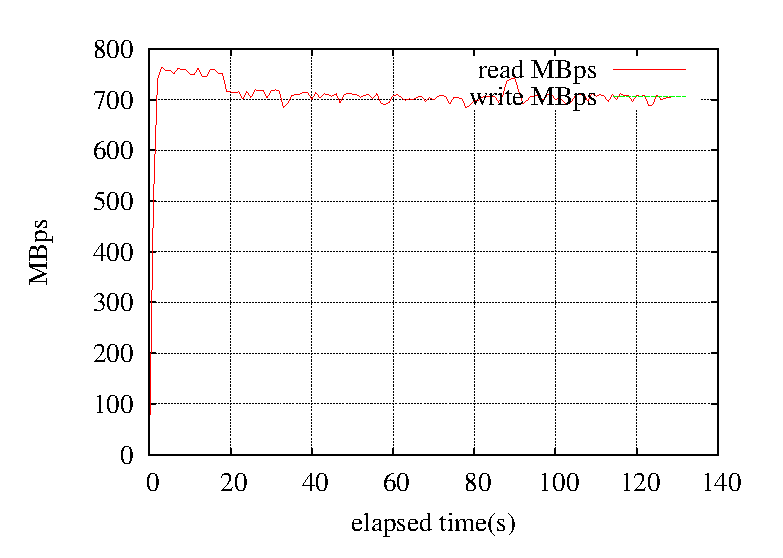
\includegraphics[width=75mm]{countlineitemmbps.eps}
  \label{fig:node1empty}}
 \end{minipage}
  \begin{minipage}[b]{\subfigwidth}
    \subfigure[local memory : 50\% occupied]
   {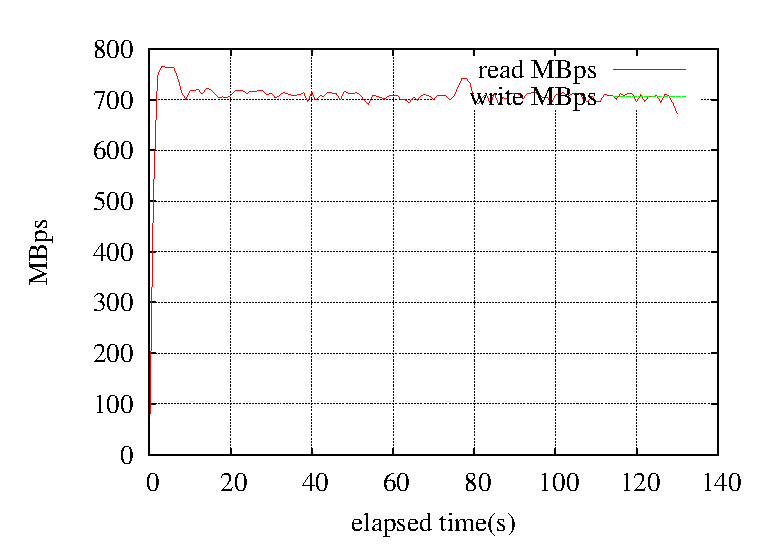
\includegraphics[width=75mm]{countlineitem_node1halfmbps.eps}
   \label{fig:node1half}}
  \end{minipage}
  \caption{MBPS}
  \label{fig:countlineitem}
\end{figure}
図\ref{fig:node1empty}と\ref{fig:node1half}でスループットが大きくなって
いる時間が大体半分程度になっている。
numactl --hardwareで一定時間おきにメモリの使用状況を追ってみても、始めに
ローカルメモリから使用されていることが確認できた。

\clearpage
\subsection{Query 1 by index scan on l\_shipdate}
lineitemのl\_shipdate attribute上にB-tree indexを構築し、
lineitem上のデータの選択率を絞って、index scanさせる。
クエリ及びクエリ実行プランは以下の通り。
\begin{description}
 \item[Query 1]\mbox{}\\
 \begin{verbatim}
 select
        l_returnflag, l_linestatus,
        sum(l_quantity) as sum_qty,
        sum(l_extendedprice) as sum_base_price,
        sum(l_extendedprice * (1 - l_discount)) as sum_disc_price,
        sum(l_extendedprice * (1 - l_discount) * (1 + l_tax)) as sum_charge,
        avg(l_quantity) as avg_qty,
        avg(l_extendedprice) as avg_price,
        avg(l_discount) as avg_disc,
        count(*) as count_order
 from
        lineitem
 where
        l_shipdate <= date '1992-02-28'
 group by
        l_returnflag, l_linestatus
 order by
        l_returnflag, l_linestatus;
 \end{verbatim}
 \item[Query execution plan]\mbox{}\\
 \small{
 \begin{verbatim}
 Sort  Sort Key: l_returnflag, l_linestatus
   ->  HashAggregate
         ->  Index Scan using l_shipdate_idx on lineitem
               Index Cond: (l_shipdate <= '1992-02-28'::date)
 \end{verbatim}
 }
\end{description}

\clearpage
\subsection{baseline計測}

\begin{figure}[thbp]
 \begin{center}
  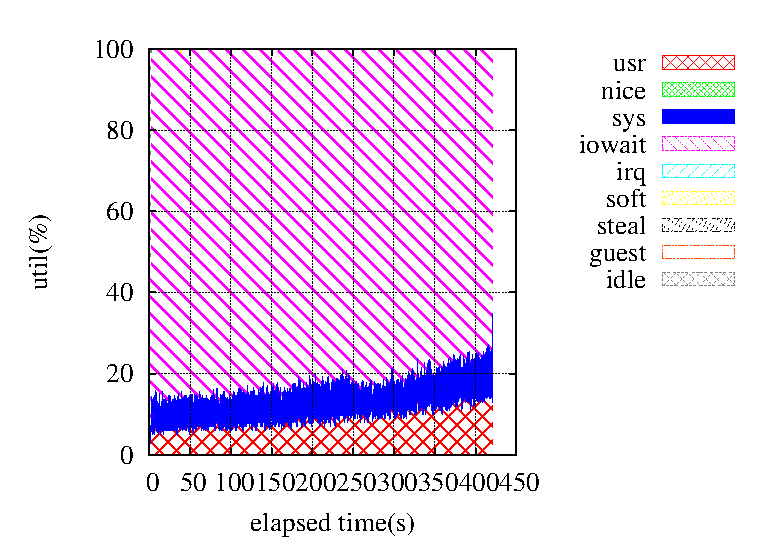
\includegraphics[width=100mm]{1idxscan_ra2048core1.eps}
 \end{center}
 \caption{cpu utilization}
 \label{fig:1idx2048core1}
\end{figure}

\begin{figure}[thbp]
 \setlength{\subfigwidth}{.5\linewidth}
 \addtolength{\subfigwidth}{-.5\subfigcolsep}
 \begin{minipage}[b]{\subfigwidth}
  \subfigure[IOPS]{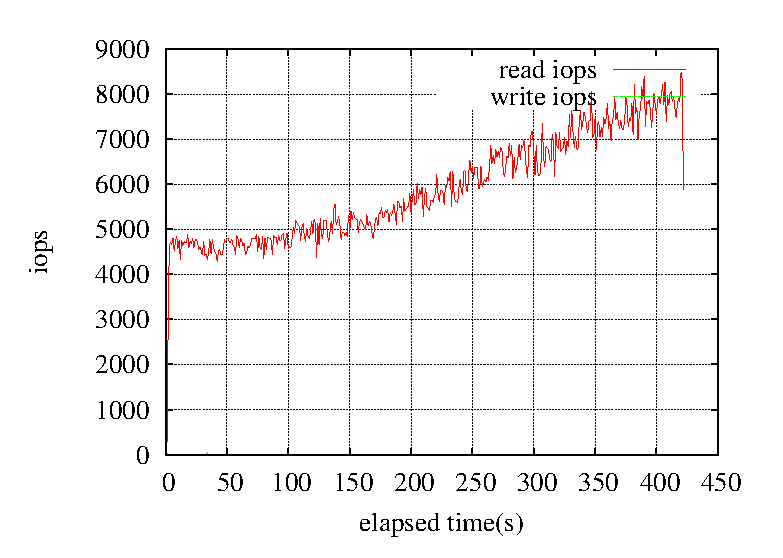
\includegraphics[width=75mm]{1idxscan_ra2048iops.eps}
  \label{fig:1idxra2048iops}}
 \end{minipage}
  \begin{minipage}[b]{\subfigwidth}
    \subfigure[MBPS]{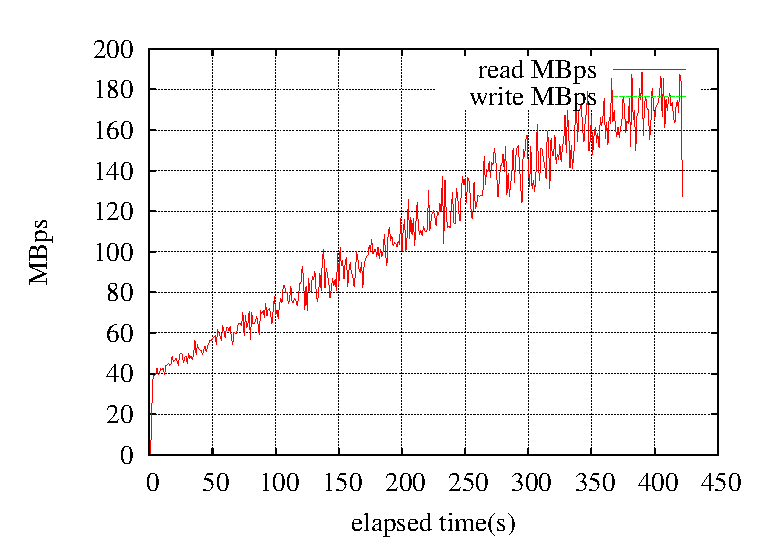
\includegraphics[width=75mm]{1idxscan_ra2048mbps.eps}
   \label{fig:1idxra2048mbps}}
  \end{minipage}
  \caption{IO spec}
n  \label{fig:1idxra2048}
\end{figure}

\begin{figure}[thbp]
 \begin{center}
  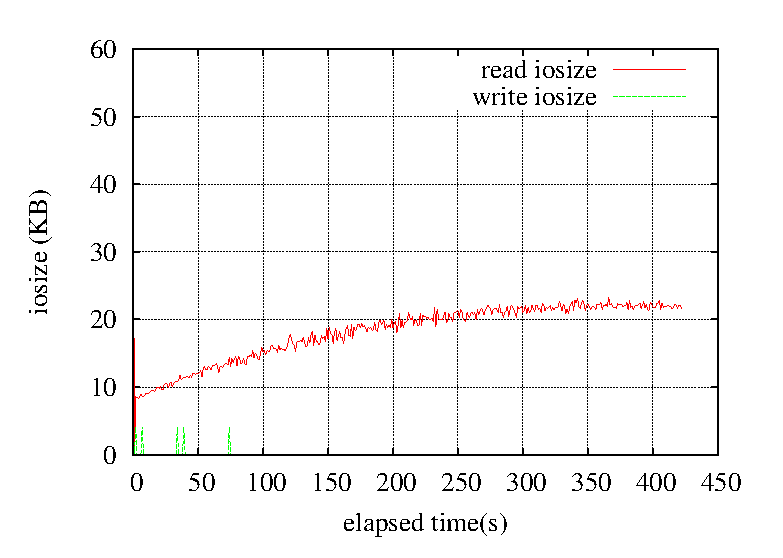
\includegraphics[width=75mm]{1idxscan_ra2048iosize.eps}
 \end{center}
 \caption{IO size}
 \label{fig:1idx2048iosize}
\end{figure}

時間の経過と共に徐々にスループットが増加しているが、IOsizeの増加から、
look-aheadの効果ではないかと考えられる。

\subsection{look-aheadをoffにした場合}
blockdev --setra 0でデバイスに対するlook-aheadを切って測定する。
\begin{figure}[thbp]
 \begin{center}
  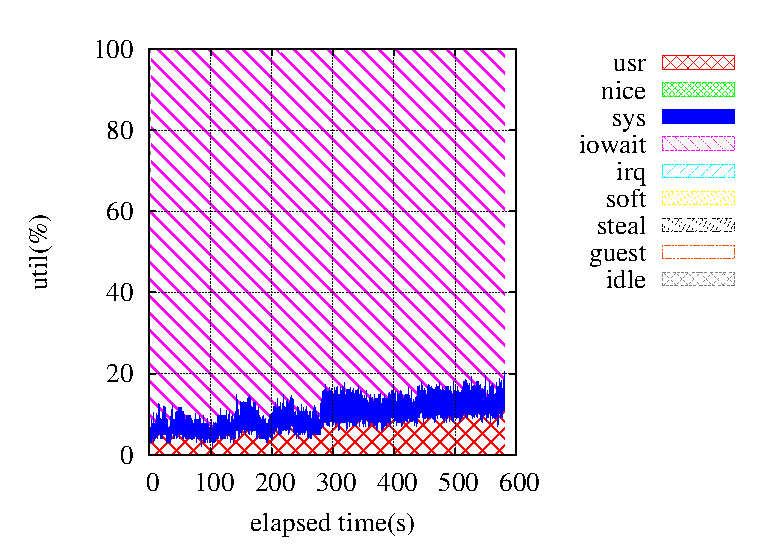
\includegraphics[width=100mm]{1idxscan_ra0core1.eps}
 \end{center}
 \caption{cpu utilization}
 \label{fig:1idx0core1}
\end{figure}

\begin{figure}[thbp]
 \setlength{\subfigwidth}{.5\linewidth}
 \addtolength{\subfigwidth}{-.5\subfigcolsep}
 \begin{minipage}[b]{\subfigwidth}
  \subfigure[IOPS]{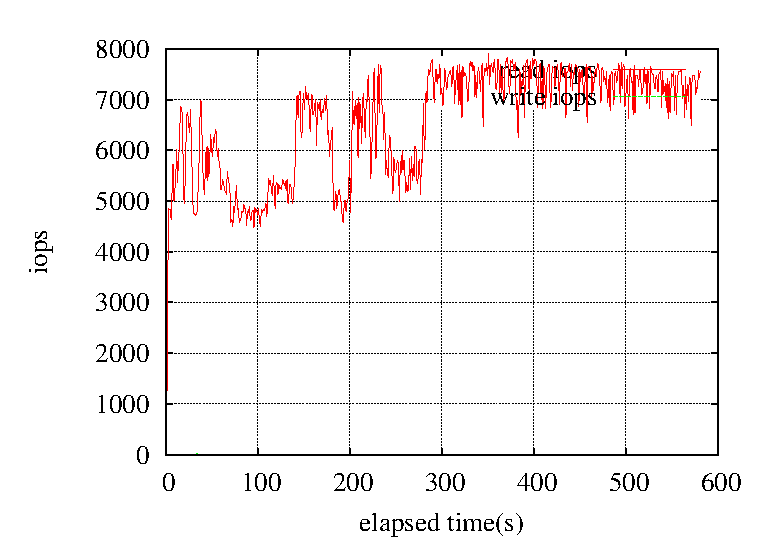
\includegraphics[width=75mm]{1idxscan_ra0iops.eps}
  \label{fig:1idxra0iops}}
 \end{minipage}
  \begin{minipage}[b]{\subfigwidth}
    \subfigure[MBPS]{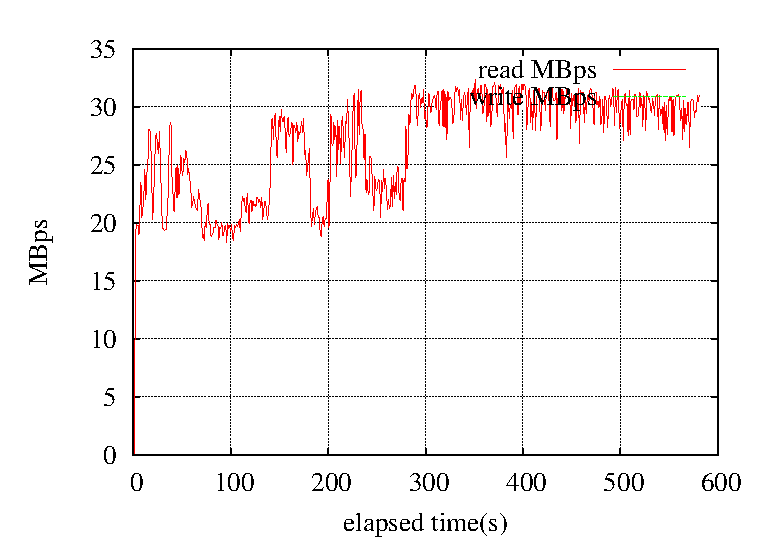
\includegraphics[width=75mm]{1idxscan_ra0mbps.eps}
   \label{fig:1idxra0mbps}}
  \end{minipage}
  \caption{IO spec}
  \label{fig:1idxra0}
\end{figure}

\begin{figure}[thbp]
 \begin{center}
  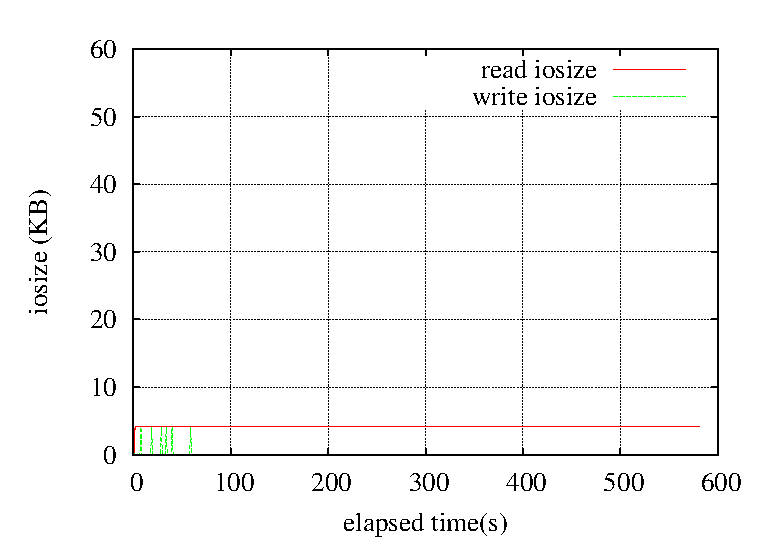
\includegraphics[width=75mm]{1idxscan_ra0iosize.eps}
 \end{center}
 \caption{IO size}
 \label{fig:1idx0iosize}
\end{figure}


\end{document}
